\hypertarget{selectmapInterface_8h}{
\section{selectmap\-Interface.h File Reference}
\label{selectmapInterface_8h}\index{selectmapInterface.h@{selectmapInterface.h}}
}
{\tt \#include $<$linux/types.h$>$}\par


Include dependency graph for selectmap\-Interface.h:\begin{figure}[H]
\begin{center}
\leavevmode
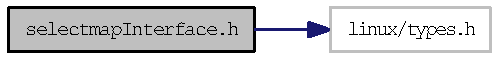
\includegraphics[width=138pt]{selectmapInterface_8h__incl}
\end{center}
\end{figure}


This graph shows which files directly or indirectly include this file:\begin{figure}[H]
\begin{center}
\leavevmode
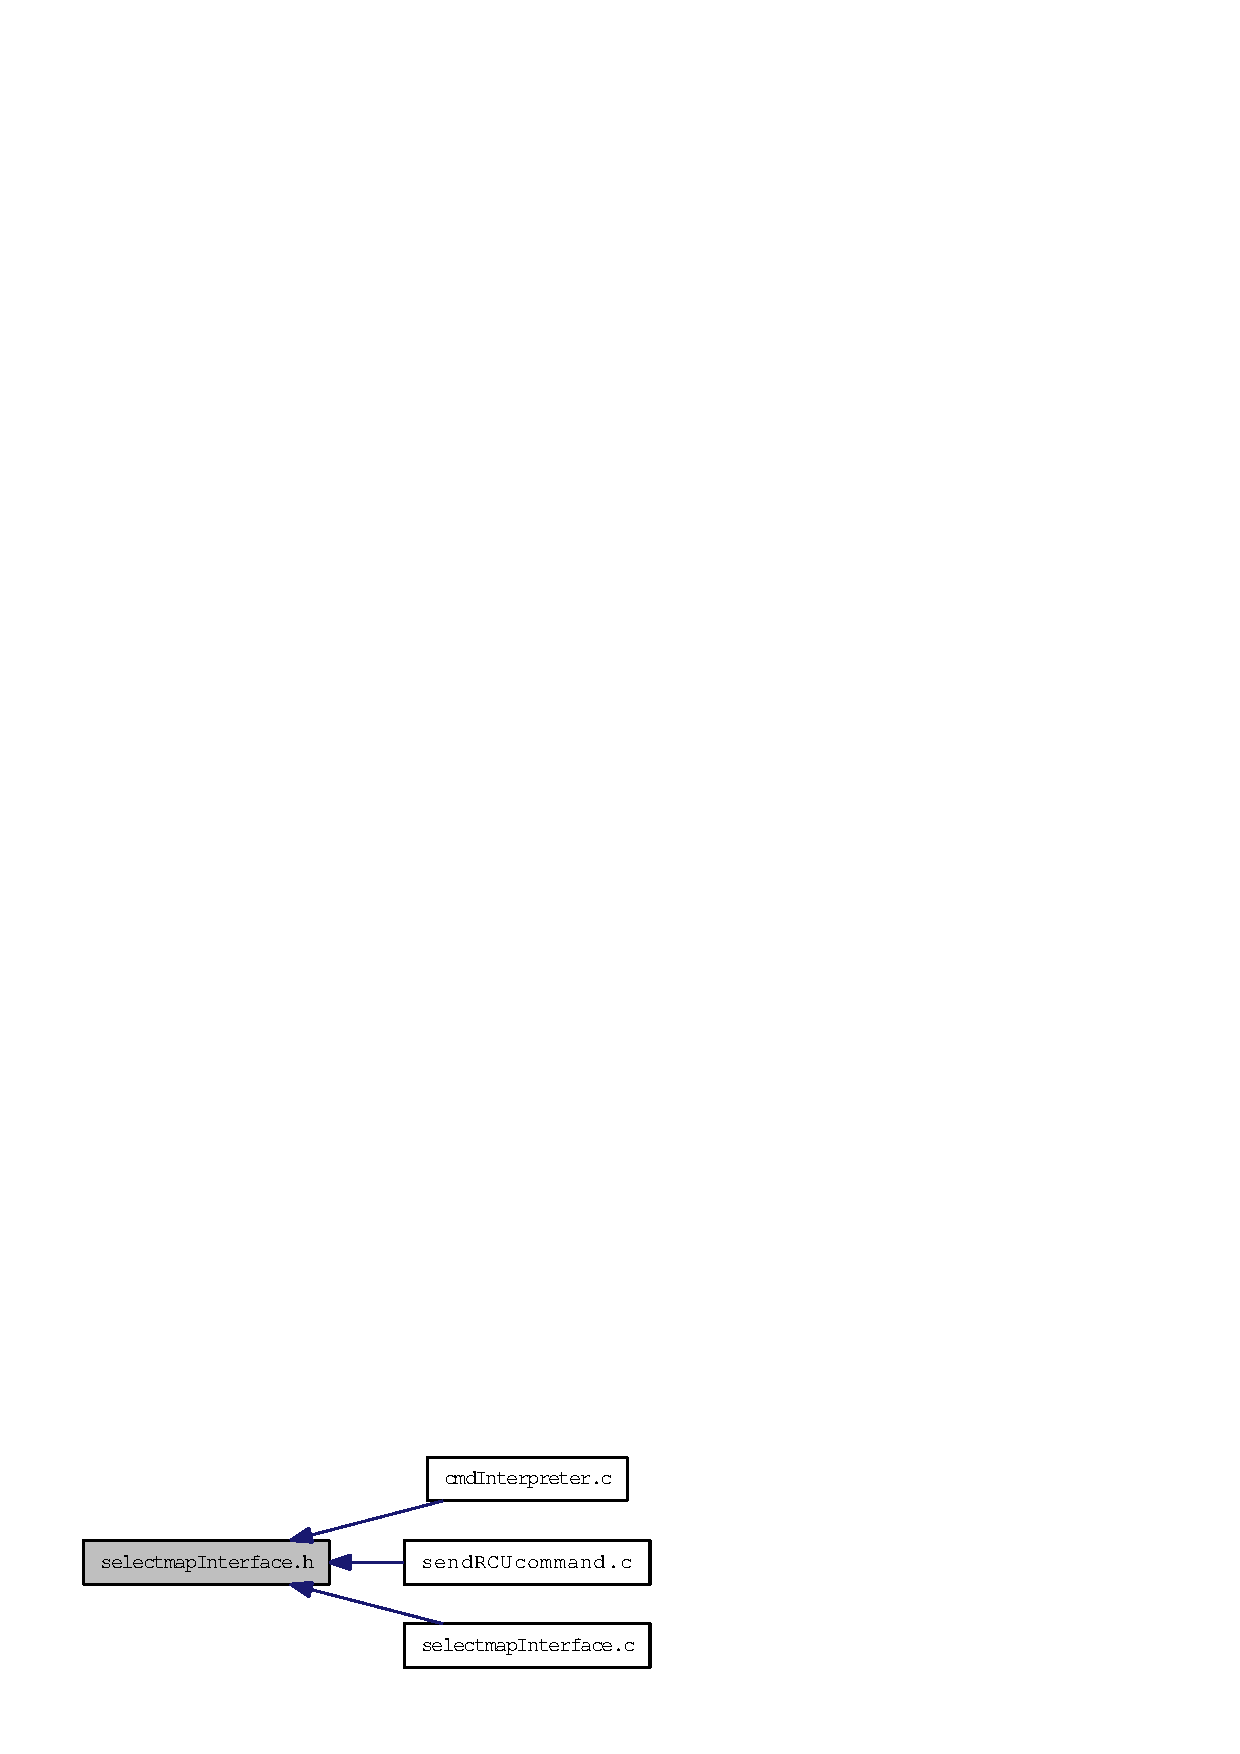
\includegraphics[width=158pt]{selectmapInterface_8h__dep__incl}
\end{center}
\end{figure}
\subsection*{API methods: Initialization and general methods.}
\begin{CompactItemize}
\item 
int \hyperlink{group__selectmap__access_g3a82967a2ac2933832a98aa2d822fd7b}{init\-Sm\-Access} (const char $\ast$p\-Device\-Name)
\begin{CompactList}\small\item\em Initialize the interface. \item\end{CompactList}\item 
int \hyperlink{group__selectmap__access_g75466b7556397eb41108eb84212c5b19}{release\-Sm\-Access} ()
\begin{CompactList}\small\item\em Close the device and release internal data structures. \item\end{CompactList}\end{CompactItemize}
\subsection*{Read/write access}
\begin{CompactItemize}
\item 
\_\-\_\-u32 \hyperlink{group__selectmap__access_g88f0784ea00a5707d5fc4db2778e1b2a}{sm\-Make\-T1Header} (\_\-\_\-u8 rdwr, \_\-\_\-u16 address, \_\-\_\-u16 words)
\begin{CompactList}\small\item\em Generates a Type 1 Header Package to send to the selectmap interface. \item\end{CompactList}\item 
int \hyperlink{group__selectmap__access_ge0d7561e2ddca5878fe0c39c948dfdd2}{sm\-Register\-Write} (\_\-\_\-u32 address, \_\-\_\-u32 data)
\begin{CompactList}\small\item\em Write one word to a register of the selectmap interface. \item\end{CompactList}\item 
int \hyperlink{group__selectmap__access_gf7536588344d4c30f928de00a240baa8}{sm\-Register\-Read} (\_\-\_\-u32 address, \_\-\_\-u32 $\ast$p\-Data)
\begin{CompactList}\small\item\em Read one word in a register of the selectmap interface. \item\end{CompactList}\end{CompactItemize}
